\pdfoutput=1
\documentclass[a4paper,11pt,titlepage, twoside]{article}

\usepackage[english]{babel}
\usepackage[utf8]{inputenc}
\usepackage{amssymb,amsmath}
\usepackage{algorithm,algpseudocode}
\usepackage[title,titletoc]{appendix}
\usepackage{latexsym}
\usepackage{a4wide}
\usepackage{color} 
\usepackage{indentfirst}
\usepackage{graphicx}       %%% graphics for dvips
\usepackage{fancyhdr}
\usepackage{longtable}
\usepackage{pifont}
\usepackage{makeidx}
\usepackage{lastpage}
\usepackage{multirow}
\usepackage{dcolumn} 
\usepackage{epstopdf}
\usepackage{url}
\usepackage{listings}
\usepackage{caption}
\usepackage{subcaption}
\usepackage{relsize}
\usepackage{pdfpages}
\usepackage{natbib}
\usepackage{url}
\usepackage{pgfplots}
\usepackage{tabularx}% http://ctan.org/pkg/tabularx
\usepackage{pgf}
\usepackage{tikz}
\usepackage[utf8]{inputenc}
\usetikzlibrary{arrows,automata,shapes,arrows, positioning, calc}

\tikzset{
    state/.style={
           rectangle,
           rounded corners,
           draw=black, very thick,
           minimum height=2em,
           inner sep=2pt,
           text centered,
           },
    nothing/.style={
           rectangle,
           rounded corners,
           draw=white, very thick,
           minimum height=2em,
           inner sep=2pt,
           text centered,
           },
}

\newcommand{\Author}{Tomáš Báča}
\newcommand{\Title}{Model predictive control of micro aerial vehicle using onboard microcontroller}
\newcommand{\Acronym}{Acronym}
\newcommand{\WorkPackage}{WorkPackage}
\newcommand{\DocName}{Master's Thesis}
\newcommand{\Subject}{\WorkPackage - \DocName}
\newcommand{\Keywords}{mobile robotics}
\newcommand{\Date}{11/05/2015}
\newcommand{\DOCVersion}{1.0}

% European layout (no extra space after `.')
\frenchspacing

% nastavení výstupu
\def\nothtml{}  					%%% \nothtml is defined if not processed with latex2html
\usepackage[                		%%% hyper-references for ps2pdf
bookmarks=true,%                   	%%% generate bookmarks ...
breaklinks=true,%                  	%%% breaks lines, but links are very small
hypertexnames=false,%              	%%% needed for correct links to figures
colorlinks=false,%
urlcolor=blue
]{hyperref}           				%%% blue instead of cyan URLS
\hypersetup{
pdfcreator  = {LaTeX with hyperref package},
pdfproducer = {dvips + ps2pdf},
}

\hypersetup{  
pdfauthor={\Author},
pdftitle={\Title - \Acronym},
pdfsubject={\Subject},
pdfkeywords={\Keywords}
}

% úpravy vzhledu stránek
\setlength{\headheight}{18pt}			%%% drobně odsadí hlavičku
\renewcommand{\footrulewidth}{0.4pt}  	%%% horizontal line in footer
\fancyhead[R]{} 						%%% umaže pravou stranu hlavičky

% řádkování
\renewcommand{\baselinestretch}{1.1}

\begin{document}

%%
%% dát pryč z elektronické verze!!
%%\setlength{\oddsidemargin}{+0.5cm} 
%%\setlength{\evensidemargin}{-0.5cm}
%%

% Titulní stránka
\pagestyle{plain}

\begin{titlepage}
\begin{center}

{\Large CZECH TECHNICAL UNIVERSITY IN PRAGUE}
\vskip 10pt

\vskip 8pt
{\Large Faculty of Electrical Engineering}
 
\vspace{50pt}
{\Huge\bf MASTER'S THESIS}\\
\vspace{40pt}

\includegraphics[width=10cm]{fig/lev.pdf}

\vspace{40pt}
{\Large\rm \Author } \\
\vspace{20pt}
{\Large\bf \Title}

\vspace{60pt}
{\bf Department of Cybernetics}\\
\vspace{5pt}   
{Thesis supervisor: {\bf Dr. Martin Saska}}

\vspace{30pt}
\end{center}
\end{titlepage}

\pagestyle{empty}
\cleardoublepage

%%
%% dát pryč z elektronické verze!!!
%%~\vfill{}

\section*{Prohlášení autora práce}
Prohlašuji, že jsem předloženou práci vypracoval samostatně a že jsem uvedl veškeré použité informační zdroje v souladu s Metodickým pokynem o dodržování etických principů při přípravě vysokoškolských závěrečných prací.

\vspace{1.5cm}
~\\

V Praze dne.............................\hfill{}...............................................

\hfill{}~~~~~~~~~~~~~~~

\newpage{}

%%\cleardoublepage
%%

%%
%% dát pryč před tiskem!!!
%~\vfill
%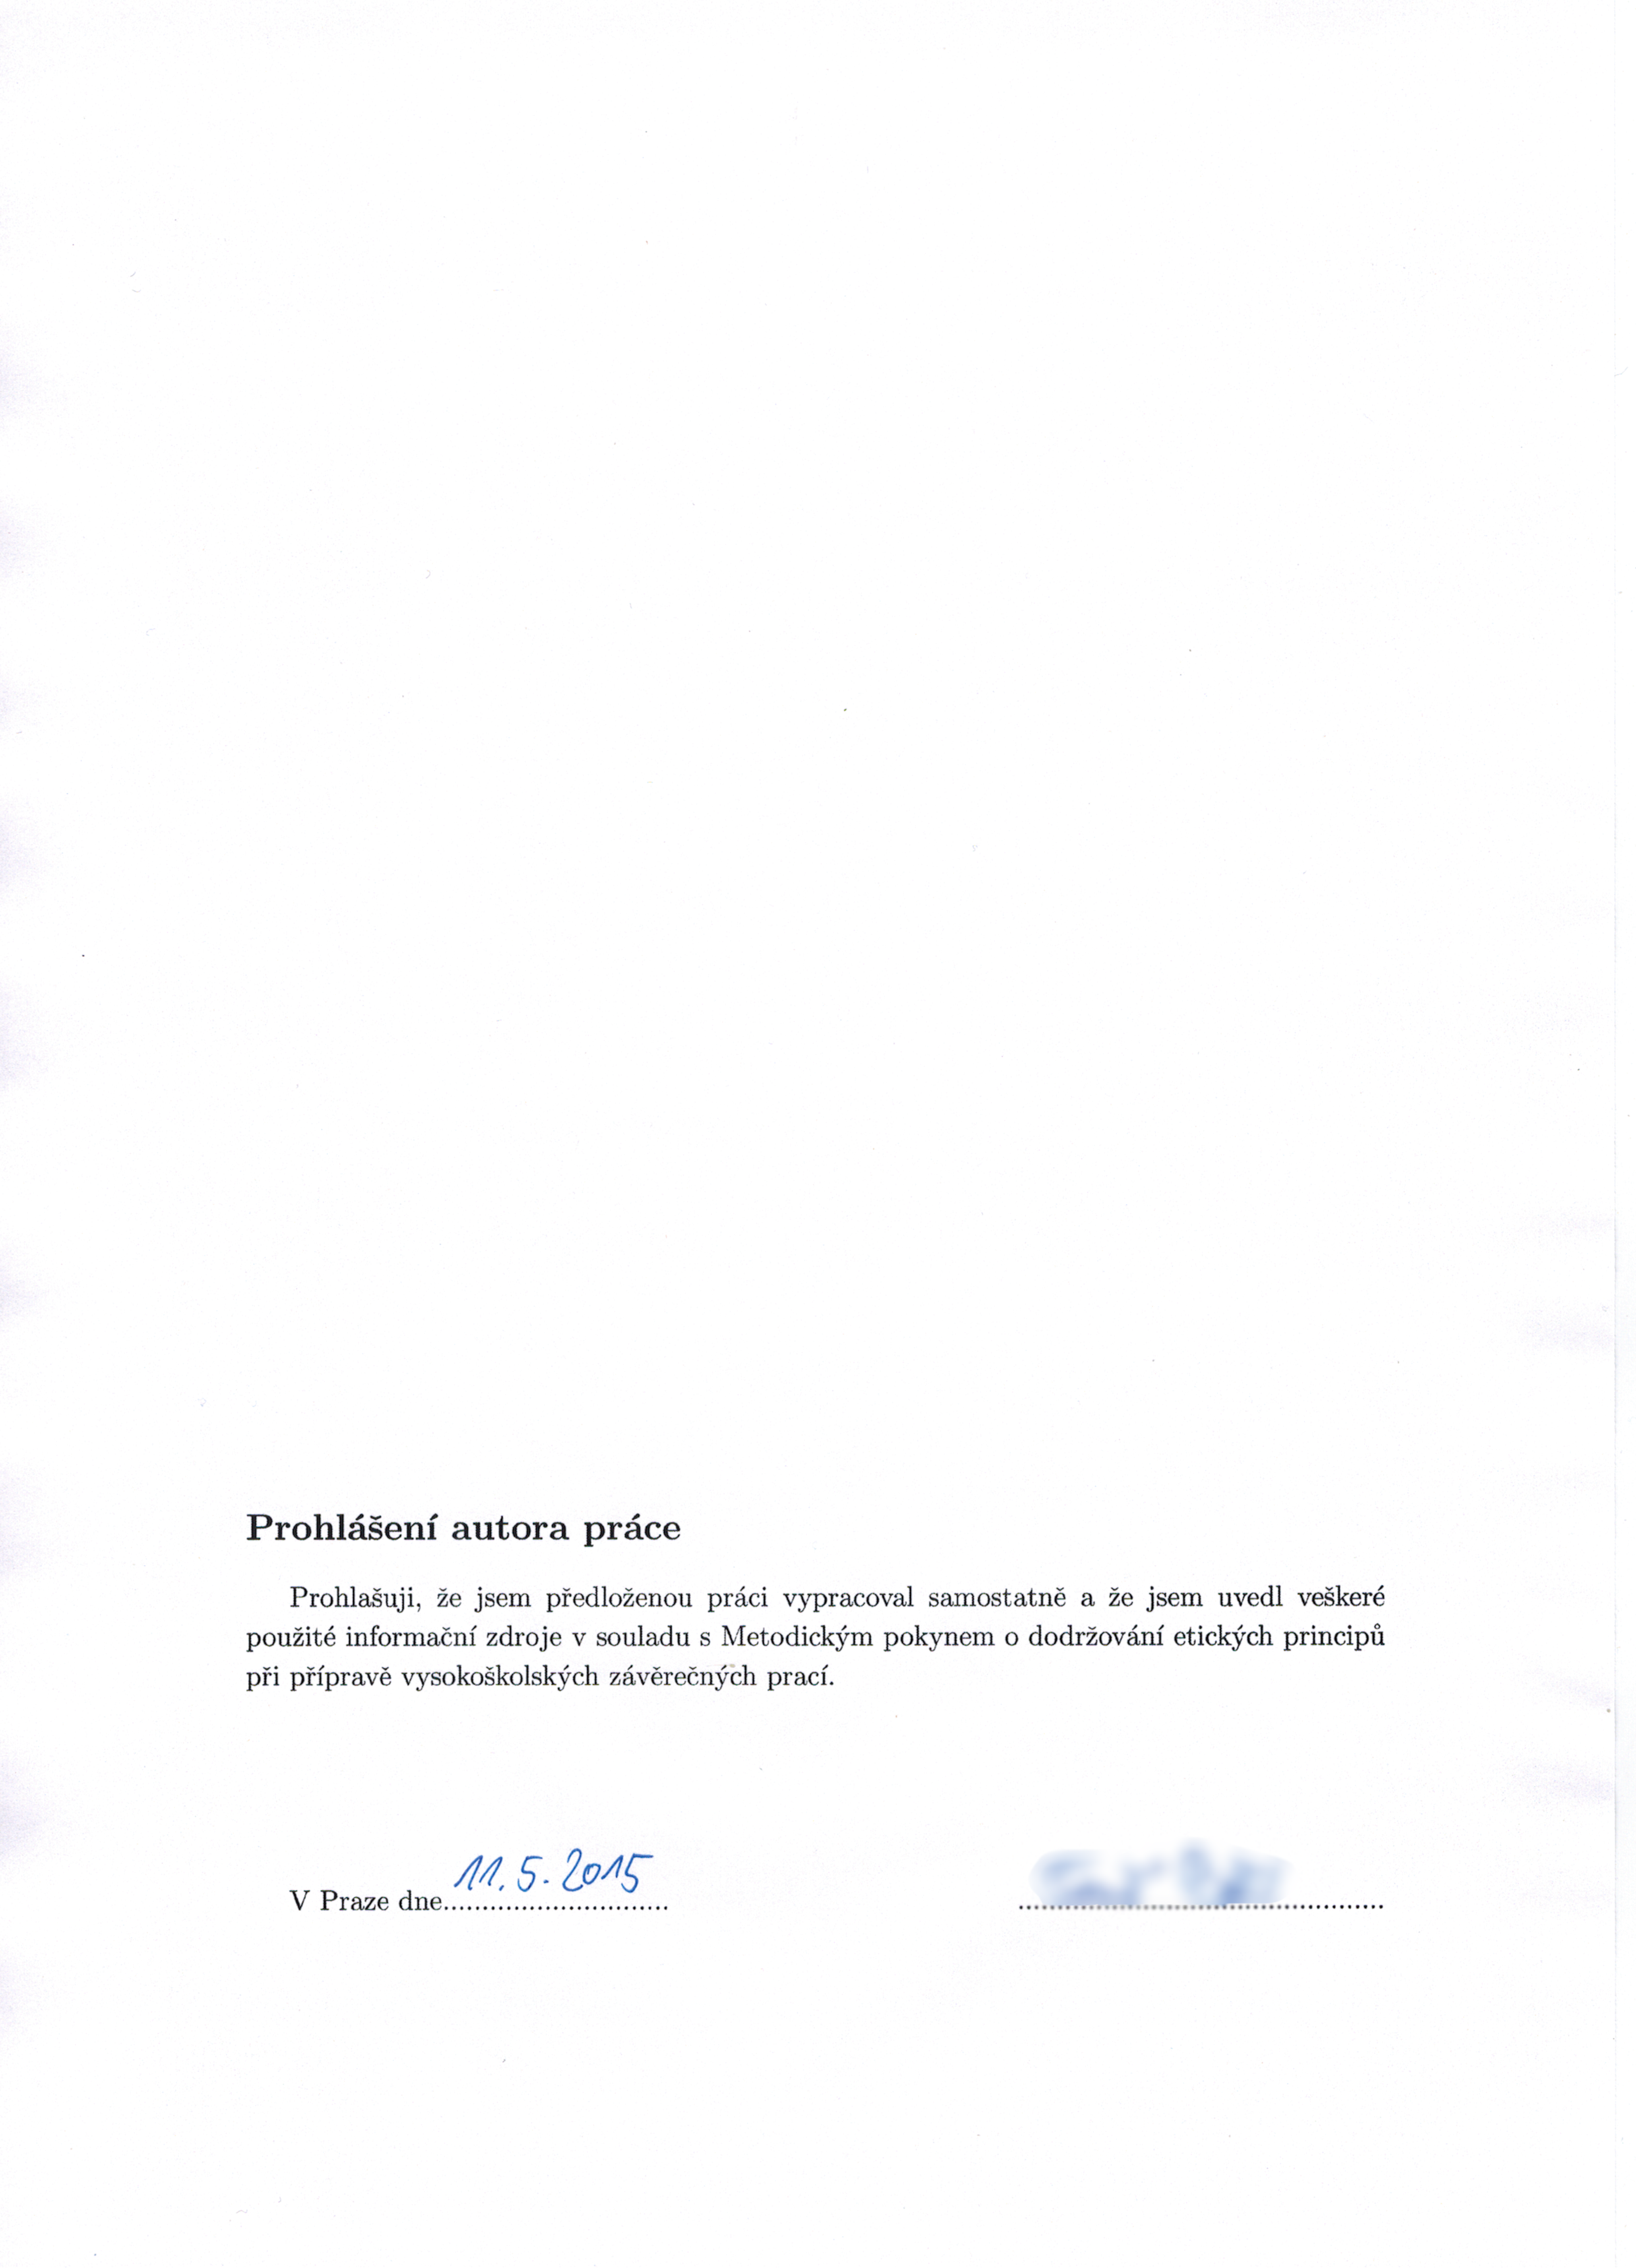
\includegraphics[width=1\textwidth]{prohlaseni.jpg}
%\cleardoublepage
%%

%% dát pryč před tiskem!!!
%\includepdf[pages={1}]{zadani_cesky.pdf}
%\cleardoublepage
%\includepdf[pages={1}]{zadani_anglicky.pdf}
%\cleardoublepage
%%

% Podekování
~\vfill{}

\section*{Acknowledgements}

Firstly I would like to thank to my family for their encouragement and support during my whole studies. Furthermore, I thank to my supervisor Martin Saska for his great support throughout this project. Finally, my thanks goes to my friend and colleague Antonín Novák for his excellent expertise and corrections regarding to mathematics.

\vspace{2.5cm}

\newpage{}

\cleardoublepage

% Stránka s abstrakty
\vfill
\begin{center}
{\it \large Abstract}
\vspace{0.2cm}

\begin{minipage}{0.8\textwidth}{
This thesis deals with automatic control of unmanned multirotor aircraft using a model predictive control approach. The focus is on design and implementation of an embedded platform to allow onboard execution of the controller. We propose a model of a dynamical system, identification of its parameter and design of a state observer. A quadratic model predictive controller is derived and implemented into the hardware, created for this purpose. Presented experiments, conducted both indoors and outdoors, proved system's capability to accurately follow a desired trajectory in space. 
}
\end{minipage}
\end{center}
\vfill
\vspace{1cm}

\vfill
\begin{center}
{\it \large Abstrakt}
\vspace{0.2cm}

\begin{minipage}{0.8\textwidth}{
Tato práce se zabývá návrhem řídicího systému pro vícerotorovou bezpilotní helikopteru s použitím metody prediktivního řízení. Za cíl si klade vývoj vestavěného systému, který umožní výpočet regulátoru přímo na palubě letounu. Předkládáme model dynamického systému helikoptery, identifikaci jeho parametrů a následný návrh pozorovatele stavů. Následuje odvození kvadratického prediktivního regulátoru a jeho implementace do navrženého hardwaru. Prezentované experimenty, provedené uvnitř i vně budovy, prokázaly schopnost přesného sledování trajektorií v prostoru.
}
\end{minipage}
\end{center}
\vfill
\vspace{1cm}
\newpage{}
\cleardoublepage

% Zapni fancy style pro Obsah a úvodní stránky...
\pagestyle{fancy}
\pagenumbering{roman}
\cfoot{\thepage}

% Obsah
\tableofcontents
\cleardoublepage

% Seznam obrázků
\listoffigures
\cleardoublepage

% Zapni fancy style na klasické stránky
\pagestyle{fancy}
\pagenumbering{arabic}
\cfoot{}								%%% zruší čísla stránek uprostřed
\rfoot{\thepage$/$\pageref{LastPage}}	%%% čísla stránek vpravo
\setlength{\parskip}{0.35cm}
\lhead{\emph{\leftmark}}	%%%	Zapne nadpis v hlavičce na všech stránkách

% Úvod
\section{Introduction}

Unmanned aerial vehicles capable of vertical takeoff and landing have undergone a big boom in past few years. It is mainly thanks to arrival of multirotor helicopters (multicopters). Their capabilities span from being a platform for professional film makers, to toys and hobby products, up to military vehicles built for reconnaissance. These vehicles (fig. \ref{fig:quadru1}) have characteristically several propellers (typically four and more) with fixed pitch angle. The machine's mechanical design is usually simple by comparison with a classical helicopter. From the mechanical point of view it has several brushless motors with propellers mounted directly on them. There is a rigid body with utility platform, motor mounts and landing gear. They can operate in situations where the presence of a person could be hazardous (natural disasters) or they can help with work tasks which would otherwise require a very expensive solution e.g. inspection of high-voltage lines. They also find an application in situations where prior technology would not help --- archaeological imaging from low-to-mid altitude.

In most cases such aircraft requires a human operator to fly although it can offer a certain level of automatic assistance. Nowadays the global position system (GPS) receiver is embedded literally in every mobile phone thus it is no surprise that it can help with control of an unmanned aircraft (UAV) when flying outdoors. Commercially available platforms can assist with position hold or even fly to a particular location. Such technology can provide an automatic flight with precision up to $1 \jed{m}$ depending on the GPS, external conditions and the vehicle itself. The scientific community showed that there are methods to increase the precision of UAV control up to centimeters by using a better localization system than GPS (namely Vicon\footnote{Vicon is a motion capture system using multiple cameras capturing the object. http://www.vicon.com/}) and implementing advanced algorithms for automatic control \citep{brescianini2013polearobatics, kumar2010grasp}.

\begin{figure}[h]
\centering
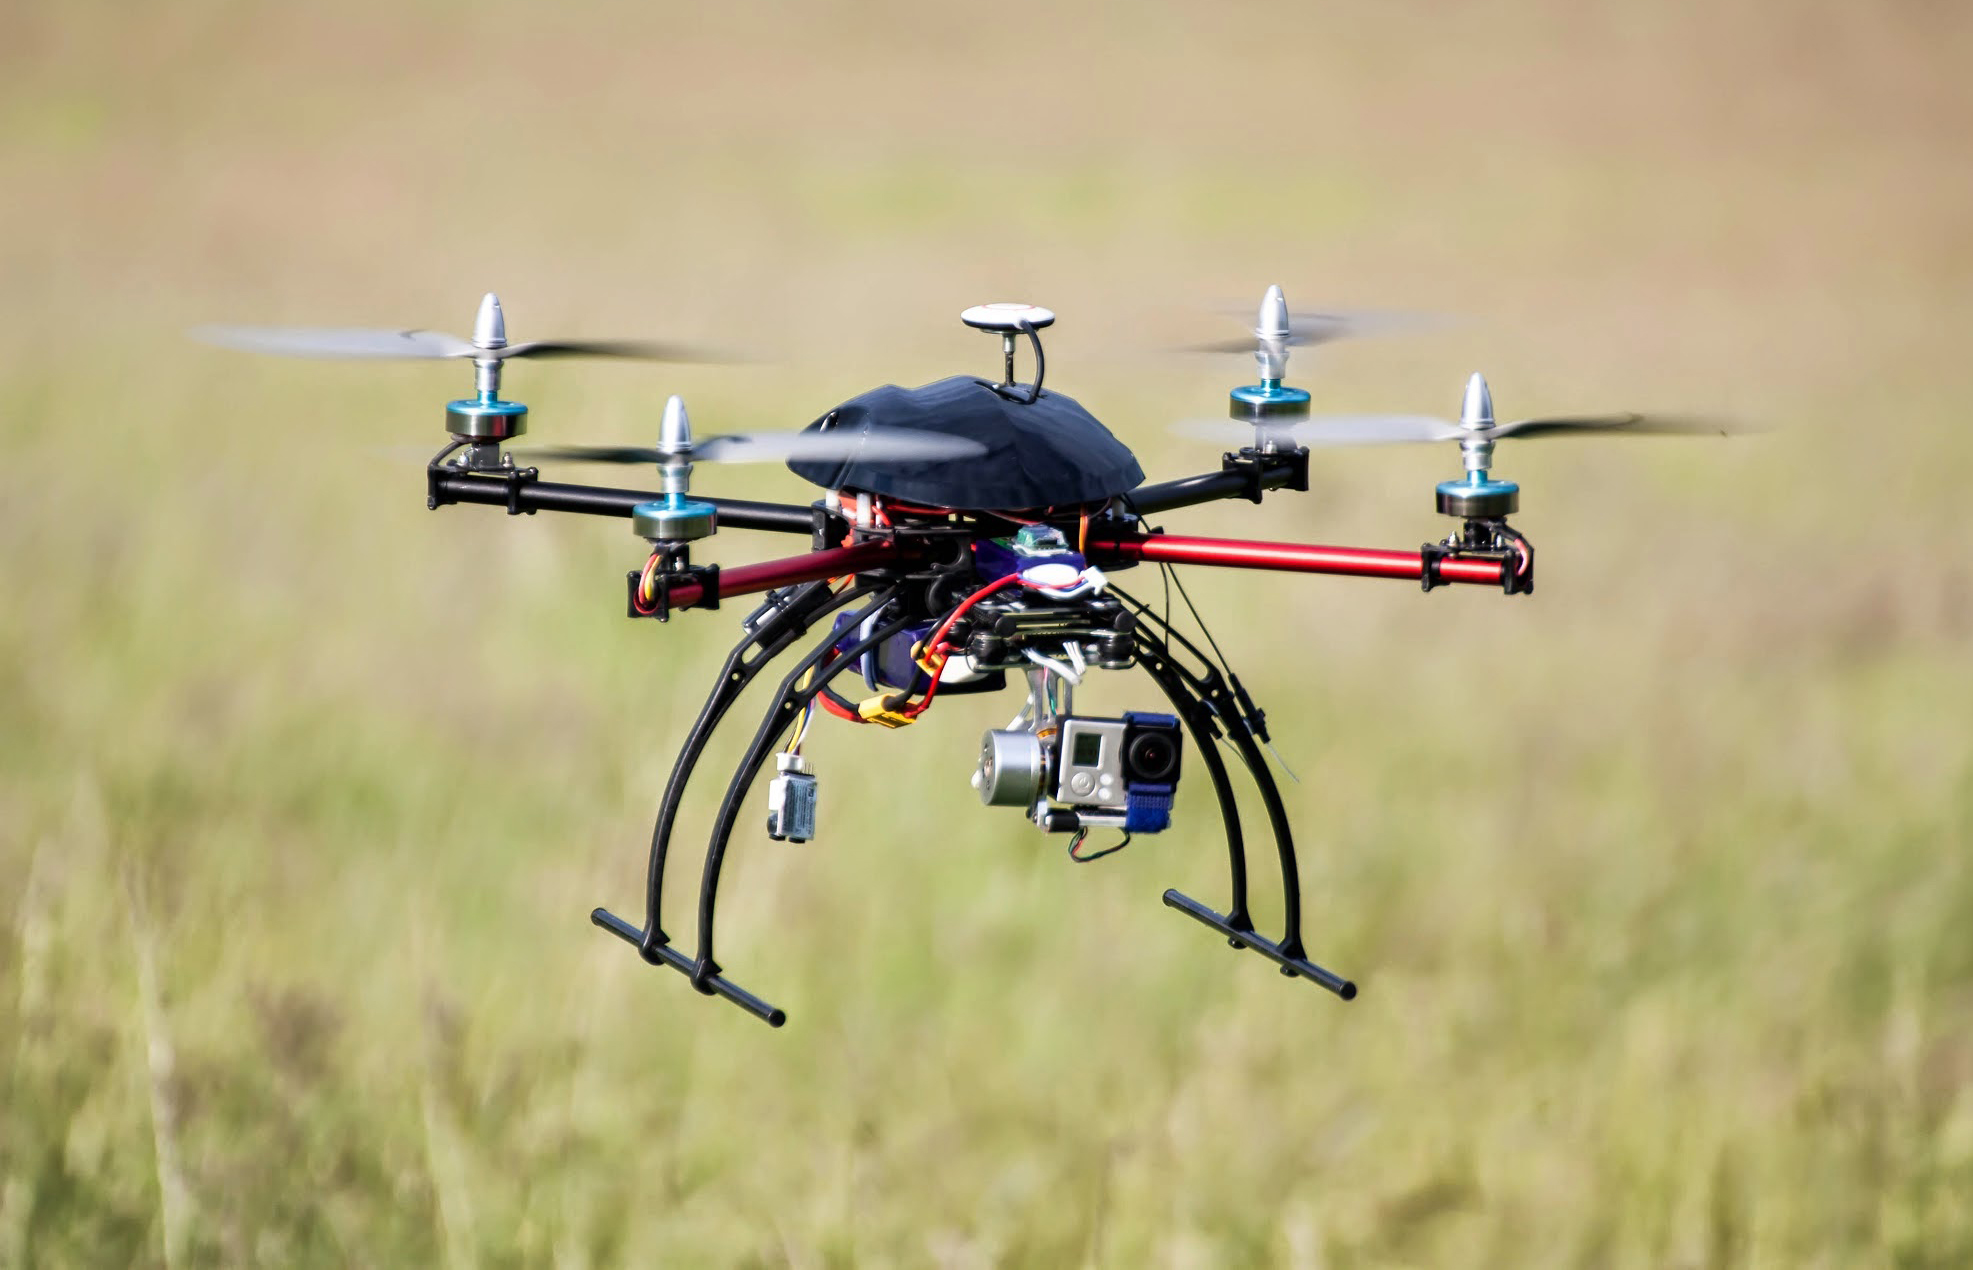
\includegraphics[width=0.75\textwidth]{fig/quadru1.jpg}
\caption{An example of multirotor aircraft used for aerial imaging.}
\label{fig:quadru1}
\end{figure}

Although the previously mentioned works required an expensive laboratory hardware and on-the-ground computational power, they can be used as an example of what one could imagine an ''automatic assistance'' would be capable of when flying indoors. Since the multirotor UAV is a highly unstable machine, feedback control is necessary to even only stop it in the air. UAVs have been a subject of research for a long time. Current intention is to build an automatic UAV that is supposed to work not only in a laboratory but also in uncontrolled indoor environment \citep{alexis2014rmpc}. A modification of current outdoor solutions for indoor usage brings new challenges and requires different approaches. The main ones are requirement of high precision control when flying indoors while omitting external localization system (like Vicon and GPS) and managing all computations onboard the vehicle itself.

The control mechanism used in today's control systems is usually satisfactory when the precision is roughly defined by the GPS localization and the control settling time is slow. It is often narrowed to PID (proportional-integral-derivative controller) that is relatively easy to compute on common embedded hardware \cite{pixhawk, ardupilot}. But when increasing requirements on precision and settling time, such approach seems to suffer if controlling this kind of unstable vehicle (see prior work in chapter \ref{cap:prior_work}). Also when imposing a requirement not only to stabilize the vehicle (stop it   from moving) but to fly through a desired space trajectory, the need for a better control design approach emerges.

One of them is a model predictive control (MPC) which is a method based on the knowledge of a dynamical model of the controlled system. It formulates the computation of control actions as a mathematical optimization problem. Mathematical optimization can solve such problems by finding a minimum of a mathematical function. MPC uses a general prediction of system future states to formulate the objective function to be optimized. There are various types of optimization problems based on the shape of the objective function and the range of its parameters. MPC is usually formulated as a continuous optimization with a convex quadratic objective function where the function itself penalizes squares of deviations from a desired state trajectory. When the optimum is found it guarantees that control actions will lead to an optimal future trajectory with respect to the objective function.

Several important features set the MPC apart from other control techniques such as PID. Firstly, it works with the state space representation of the system and all states (e.g. position, velocity, acceleration, ...) participate as an input for optimization, not only a control error of the tracked state (usually position) as it is with the PID. Although, there are methods for nesting multiple controllers, the MPC offers a direct way to work with all states of the system. The other important feature is the way in which MPC handles constraints. We can impose constraints on inputs, systems states and even more complex ones. Though the optimization task becomes more complicated --- linearly constrained convex quadratic optimization, it still has a global optimum which can be found in reasonable time. Another feature is a capability to account in disturbances. When properly modeled and estimated, a disturbance can be used directly by the controller to produce adequate control actions.

As it was previously mentioned, MPC has been already successfully used for control of UAVs. But the challenging task is to implement it solely on the hardware onboard of the UAV where computational power is very limited. Today microcontrollers{A microcontroller is an integrated circuit containing a processor, operating memory, program memory and peripheral controller.} can have parameters similar to $\approx 200 \jed{MHz}$ clock, $\approx 200 \jed{kB}$ RAM and mainly floating point performance in order of $10^7$ operations per second. Surely one could ask, why not to equip the UAV with a dedicated (miniaturized) PC to handle the computation. Our goal is to create a small all-in-one solution which can be mounted on any micro aerial vehicle (MAV) where the potential payload capacity could be only hundreds of grams. In the long term this would allow us to create a swarm of self-sustained MAVs that could solve tasks as remote sensing, localization of dangerous objects or mapping even in indoor and unknown environment.

POPIS VŠECH PRACÍ OD STAVBY HELIKOPTERY K EXPERIMENTŮM

CO BUDE VE KTERÝCH ČÁSTECH PRÁCE

\subsection{Problem statement}

The task of this thesis is to design, build and implement an embedded controller that will utilize the model predictive control approach to drive the aircraft in a way suitable for indoor use, supporting precise trajectory following, and in future enabled its usage in formations and swarms of helicopter. It entails a design and creation of dedicated circuit board which will allow to work with any usual UAV and extends its capabilities to fulfill complex robotic tasks. It should support connecting a variety of external peripherals and sensors to localize the helicopter in space. Firstly, system modeling and identification need to be done to supply a dynamical model for simulation purposes and the MPC itself. It is followed up by a design of a state observer to track the current position of the UAV based on its sensors and to estimate all other states for purpose of the MPC. The design of the model predictive controller requires a formulation of optimization task

\begin{equation}
\label{eq:qmpc_intro}
\begin{aligned}
& \min_{\textbf{x} \in \mathbb{R}^{N}}
& & \mathrm{J}(\textbf{x}) = \frac{1}{2}\textbf{x}^T\textbf{H}\textbf{x} + \textbf{x}^T\textbf{c}\\
& \text{s.t.}
& & \text{constrains on \textbf{x}},
\end{aligned}
\end{equation}
\\
where \textbf{x} is the solution that leads to the desired control actions over a certain \emph{prediction horizon}. A proper method for solving the optimization process need to be chosen and implemented on the embedded hardware of the UAV. Previously mentioned tasks should be accompanied by simulation of the system including modeling of measurements, data filtration and the flight itself. There are minor tasks tied to the implementation and hardware design, mainly resolving communication, signal processing, data handling. The final outcome should be verified using variety of experiments testing its capabilities and finally compared to the prior solution used in the laboratory up to now.

\subsection{Previous work}
\label{cap:prior_work}

There has been a research on UAV control in laboratory of Intelligent and Mobile Robotics (IMR) group at FEE CTU Prague since 2011. The main focus has been on simulation of relatively localized UAV swarms and formations. Because it was also desired to verify the results experimentally, a development of hardware platform started. The first experiments has been done with AR Drone platform \citep{kranik2012drone} but it was shown that there is a need for a customizable platform capable of lifting heavier payload.

The first iteration of creating the custom platform is depicted in \citep{baca2013}. A custom control board was developed accommodating PID controllers. It could be mounted on a general purpose UAV and allowed connecting a dedicated onboard camera localization system \citep{faigl2013low}. Experiments showed that the UAV is able to track and follow the position of a ground robot marked for image recognition. It was also tested that localization based solely on the position of a moving object (another robot or UAV) tends to destabilize the vehicle. Experiments were conducted with a heterogeneous formation of two helicopters and one ground robot.

Subsequent work has been done in \citep{endrych2014} utilizing the same hardware accompanied by the \textit{px4flow} optical flow sensor. PID controllers were fine-tuned and the system was further improved to allow automatic flight even when the tracked object cannot be seen. This allowed creating formations of multiple UAVs which was not successful with the former system. Experiments were again conducted to test the system's performance.

Furthermore, the need for a precise execution of indoor experiments led to increasing focus in development of the control system itself. This thesis describes a development of new hardware platform which satisfies demands that arose during the previous work. The system should be capable of executing a MPC controller, transmitting telemetry to ground station as well as logging data onboard in realtime. 

\subsection{Related work}

It is difficult to find results on completely embedded MPC control of UAV. Those who are not only scientifically active in simulating flight control but verify their outcomes experimentally tend to use an external localization system and on the ground computational power, since it makes experiments much less demanding on particular hardware implementation. Following survey contains the state of the art of both, embedded and ground computed MPC.

The paper \citep{bangura2014realtimempc} shows an onboard quadratic implementation of MPC running on Pixhawk platform \citep{pixhawk}. The control problem with the prediction horizon of length 5 steps is solved by unconstrained optimization. The UAV is supplied with position data gathered from the Vicon system and transmitted to the vehicle wirelessly. Data from presented experiments suggest that the aircraft is capable of tracking position step changes and harmonic trajectory. A correct MPC formulation is presented. The paper lacks description of experiments inc. multimedia material, which is suspicious since it presents a working and flying autonomous helicopter. The system is not fully onboard and the results can be overcome.

The paper \citep{alexis2014rmpc} is considered as the current state of the art in the field of embedded MPC implementation on UAV. Authors have proposed a solution based on RMPC (Robust MPC)  utilizing an explicit formulation of the optimization task. The RMPC takes a form of a linear objective subject to linear constraints (Linear Programming). The formulation allows a disturbance rejection which is demonstrated by experiments where the UAV follows a trajectory while being under the influence of wind gusts. The experimental platform consists of two vehicles equipped with Atom based PC, one of them being localized by Vicon, the other one equipped with a ultrasonic rangefinder and camera for computing an optical flow. The presented solution also allows to incorporate a collision avoidance directly into the control loop, which is experimentally verified in the paper. Despite the results are impressive, the approach suffers from combination of a trajectory planner and a low-level controller in one system. The overall performance of the controller (its capability to follow the trajectory) is lower than if using our approach, because the optimization takes care of creating the optimal trajectory using state constraints. Theoretical and experimental analyses show that a better approach is to separate the controller from a trajectory planner. The trajectory planner may use an MPC approach too (even non-linear \citep{saska2014formations}), but its execution rate can be slower than of the controller. See section \ref{cap:implementing_qmpc} for detailed discussion to this topic.

Another work \citep{papachristos2013} (prior to \citep{alexis2014rmpc}) shows an implementation of a quadratic MPC, embedded on tilt-rotor aircraft, utilizing onboard Atom based computer. The position of UAV is estimated from onboard sensor data. The constrained formulation presented in the paper can handle state constraints and allow optimization over prediction horizon of 8 steps. Experiments were conducted in order to show its ability to track desired 3D trajectory and reject position disturbances.

Authors of technical report \citep{bouffard2012dtic} and later paper \citep{bouffard2012learning} managed to implement the explicit formulation of quadratic MPC using onboard Atom PC. They localize the helicopter using the Vicon system and use a learning based MPC to improve the performance of the system. Their experiments involved a helicopter catching a flying ball. 

In \cite{suzuki2014collision}, a non-linear MPC formulation allowing to control several miniature, single-rotor helicopters in a collision-free way, is presented. An external camera localization system as well as a ground computer station are utilized. The MPC optimizes over $2 \jed{s}$ prediction horizon. Their simulation result has been experimentally verified with one miniature helicopter.

University ETH in Zurich has a long tradition of research in the field of UAV control. Some of their videos of helicopter aerobatics have been commonly known even among general public. They have accomplished astounding achievements with UAVs with the Vicon system involved \citep{brescianini2013polearobatics, Augugliaro2013buildingstructures}. Their contribution to MPC is published in \citep{ethMueller2013mpc}, it also relies on the external localization system as well as the PC ground station.

Almost all of presented works was implemented using a single MPC approach to control the vehicle together with creating the optimal trajectory. We aim to decompose those problems. This thesis presents MPC controller, while our other related work describes the trajectory planning \citep{saska_baca2014, saska2014formations}.

SUMARIZOVAT STATE-OF-THE-ART, ANEB ROZŠÍŘIT PŘEDCHOZÍ ODSTAVEC

\subsection{Contribution}

We present a control system for UAV that allows the execution of quadratic MPC onboard the aircraft. It consists of a single board equipped with two microcontrollers, telemetry module and SD-card data logger. The system was tested with the \textit{px4flow} optical flow sensor, but allows connecting other sensors and modules. A custom implementation of QMPC enables to control the UAV with $2.2\jed{s}$ prediction horizon. The implementation allows to estimate system disturbances with Kalman filter and reject them directly with the controller. When flying in indoor environment, the system is able to track desired trajectories with errors in order of centimeters. Experiments have shown that the results are similar to current state of the art solutions. It can be implemented in very small UAVs (5 inch propellers) to allow flying in compact formations in indoor environment. Our contribution beyond the state-of-the-art approach is summarized in following points:

\begin{itemize}
\item We formulated a system observer and MPC controller for embedded implementation.
\item We present a disturbance rejection model delivering an offset-free tracking.
\item We designed a hardware platform specifically intended for UAV MPC control relying on onboard sensors and computational resources.
\end{itemize}

\subsection{Mathematical notation}

The table \ref{tab:notation} denotes the basic mathematical notation used in this thesis.

\begin{table}[h]
\centering
\begin{tabular}{ll}
\hline
Symbol & Description \\
\hline
lower or uppercase letter, e.g. $n$, $N$ & a scalar \\
bold lowercase letter, e.g. \textbf{x} & a column vector \\ 
bold uppercase letter, e.g. \textbf{A} & a matrix \\
$\textbf{x}^T$, $\textbf{A}^T$ & vector and matrix transpose \\
underlined vector, e.g. \textbf{\underline{x}} & concatenated vectors $\left(\textbf{x}_1^T,\textbf{x}_2^T,...,\textbf{x}_n^T\right)^T$ \\
\textbf{I} & identity matrix \\
\textbf{1} & matrix of ones \\
$x^{(W)}$ & $x$ in coordinate system $W$ \\ 
$x_{[t]}$, $\textbf{x}_{[t]}$ & $x$, $\textbf{x}$ in the sample time $t$ \\
$\mathbb{R}$, $\mathbb{N}$ & set of real and natural numbers \\
\hline
\end{tabular}
\caption{Overview of mathematical notation.}
\label{tab:notation}
\end{table}


\clearpage

% State of the art
\section{Related work}

Text text, state of the art, blah blah
\clearpage

% UAV system dynamics
\section{UAV dynamics}


\clearpage

% Závěr
\section{Conclusion}

In this thesis, we developed a hardware and software solution that allows execution of the model predictive controller onboard of micro aerial vehicles. The dynamical model of the helicopter was derived and its parameters were numerically and experimentally identified. We designed a system including the Kalman filter as the state estimator and the quadratic MPC which optimizes control actions over the prediction horizon of 2.2\jed{s}. The proposed system was successfully implemented into the embedded hardware. The controller was verified by simulation and tested in various experiments. Many experiments were conducted both indoors and outdoors to test different scenarios including tracking various trajectories and disturbance rejection. The entire assignment of this thesis has been fulfilled successfully. Following tasks has been completed:

\begin{itemize}
\item The dynamical system of the UAV was analyzed and its model was constructed.
\item A Kalman filter was implemented to allow state estimation and disturbance estimation.
\item A model predictive controller was derived and implemented on the experimental micro aerial vehicle.
\item The experimental aircraft was constructed including the custom control board, which was designed and manufactured for purpose of this thesis.
\item Experiments were conducted that verified capabilities of the solution to follow dynamical trajectories in indoor and outdoor environment.
\end{itemize}

This thesis was designed to allow its extension by other students, namely \citep{klucka2015, fiedler2015}. One aimed to control a group of UAV's synchronously using the XBee modules, another developed a user interface for the ground station and dealt with a failure detection system based on proposed estimator. The platform will continue to be used for a research of UAV swarms and formations within Multi-Robot System group of FEE CTU.

The experimental platform was used during research of a visual feature tracking system \citep{chudoba2014surf}. The results with multirobotic formations were also published in \citep{saska_baca2014}. The last results were submitted to Autonomous Robots journal and are expected to come out in 2015 \citep{saska2015submitted}. 

The thesis is an outcome of a long lasting and diligent work. The author is grateful for the knowledge and experience he gained, both theoretical and technical. It is a little but important piece of the puzzle to allow autonomous operation of relatively localized unmanned aircraft. The future is in the sign of pushing frontiers of unmanned vehicles --- let us see what will it bring.

\subsection{Future work}

During the development of this thesis, several ideas and needs emerged that specify our future work. Since the bottleneck of the system is its dependence on sensor data, additional onboard sensors should be mounted to increase the precision and robustness of estimated position. Barometer and magnetometer could be added to the custom control board and their data fused by the Kalman filter. The IMU, which is already present in the stabilization board, could be also used for the position estimation.

Regarding controllers, the MPC shall be implemented to control also the altitude, although there is not such need for precise trajectory tracking. Furthermore, an additional MPC could be added to allow optimal onboard trajectory planning. It would require to solve an optimization problem with more complex constraints. 

\cleardoublepage

% Bibliografie
\bibliography{dp}{}
\cleardoublepage
\bibliographystyle{plain}
\clearpage

% Apendixy, schemata, seznam zkratek, atp...
\appendices
\lhead{\emph{APPENDIX \leftmark}} 
\section{CD Content}

In Table~\ref{tab:obsah} are listed names of directories on CD.

\vspace{1cm}
\begin{table}[!htb]
\centering
\begin{tabular}{lp{10cm}}
\hline
\textbf{Directory name} & \textbf{Description} \\
\hline
thesis & Master's thesis in pdf format\\
thesis\_sources & latex source codes \\
src/STM & sources for STM32F4 \\
src/xMega & sources for ATXMega128A3U \\
src/Matlab & matlab scripts for simulation and identification \\
src/CMatrixLib & CMatrixLib matrix library \\
src/hardware & Eagle files and material for PCB reproduction\\
videos & videos from experiments \\
\hline
\end{tabular}
\caption{CD Content}
\label{tab:obsah}
\end{table}
\cleardoublepage

\section{List of abbreviations}\label{ape:abbreviations}

In Table \ref{table:abbreviations} are listed abbreviations used in this thesis.

\begin{table}[!htb]
\centering
\begin{tabular}{ll}
\hline
\textbf{Abbreviation} & \textbf{Meaning} \\
\hline
\textbf{ANSI C} & a standard for C programming language \\
\textbf{API} & application programming interface \\
\textbf{AVR} & Atmel's micro-controller architecture \\
\textbf{ARM} & RICS processor architecture \\
\textbf{EKF} & extended Kalman filter \\ 
\textbf{ESC} & electronic speed controller \\
\textbf{FPU} & floating-point unit \\
\textbf{GNU} & GNU's not Unix \\
\textbf{GPS} & global positioning system \\
\textbf{IMU} & inertial measurement unit \\
\textbf{$\textsc{i}^2\textsc{c}$} & two-wire serial interface\\
\textbf{KF} & Kalman filter \\
\textbf{KK2} & name of used stabilization board\\
\textbf{LP} & linear programming \\
\textbf{LTI} & liner time-invariant \\
\textbf{MCU} & microcontroller unit \\
\textbf{MAV} & micro aerial vehicle \\
\textbf{MEMS} & micro-electro-mechanical system \\
\textbf{MPC} & model predictive controller \\
\textbf{PC} & personal computer \\
\textbf{PID} & proportional-integral-derivative controller \\
\textbf{PPM} & pulse-position modulation \\
\textbf{QMPC} & quadratic model predictive control\\
\textbf{QP} & quadratic programming \\
\textbf{RAM} & random access memory \\
\textbf{RC} & remotely controlled / remote controller \\
\textbf{RMPC} & robust model predictive controller \\
\textbf{RTOS} & real-time operating system \\
\textbf{SRAM} & static random access memory \\
\textbf{STM} & STMicroelectronics company \\ 
\textbf{UART} & universal asynchronous receiver transmitter \\
\textbf{UAV} & unmanned aerial aircraft \\
\hline
\end{tabular}
\caption{Lists of abbreviations}
\label{table:abbreviations}
\end{table}
\cleardoublepage

\end{document}
